\begin{frame}{Initialization}
	
Motivated by the bounds for the vanishing gradient on the singular values of the recurrent matrix we explored an initialization scheme which \textbf{scales the spectral radius} of such matrix.

\vspace{2em}

\begin{algorithm}[H]
	\KwData{\\
		\Indp
		$\rho = $ desired spectral radius
	}
	\BlankLine
	
	$\mat{W_{rec}} \sim \mathcal{N}(0, \sigma^2)$\\
	$r \gets \mbox{spectral\_radius}(\mat{W_{rec}})$\\
	$\mat{W_{rec}}\gets \frac{\rho}{r} \cdot \mat{W_{rec}}$\\
	\KwRet{$\mat{W_{rec}}$}
	\caption{Recurrent weight matrix initialization scheme}
	\label{algo:init_scaling}
\end{algorithm}
\end{frame}

\begin{frame}{Effect of initialization on the temporal gradients}
	\vspace{-3em}
	\begin{figure}[H]
		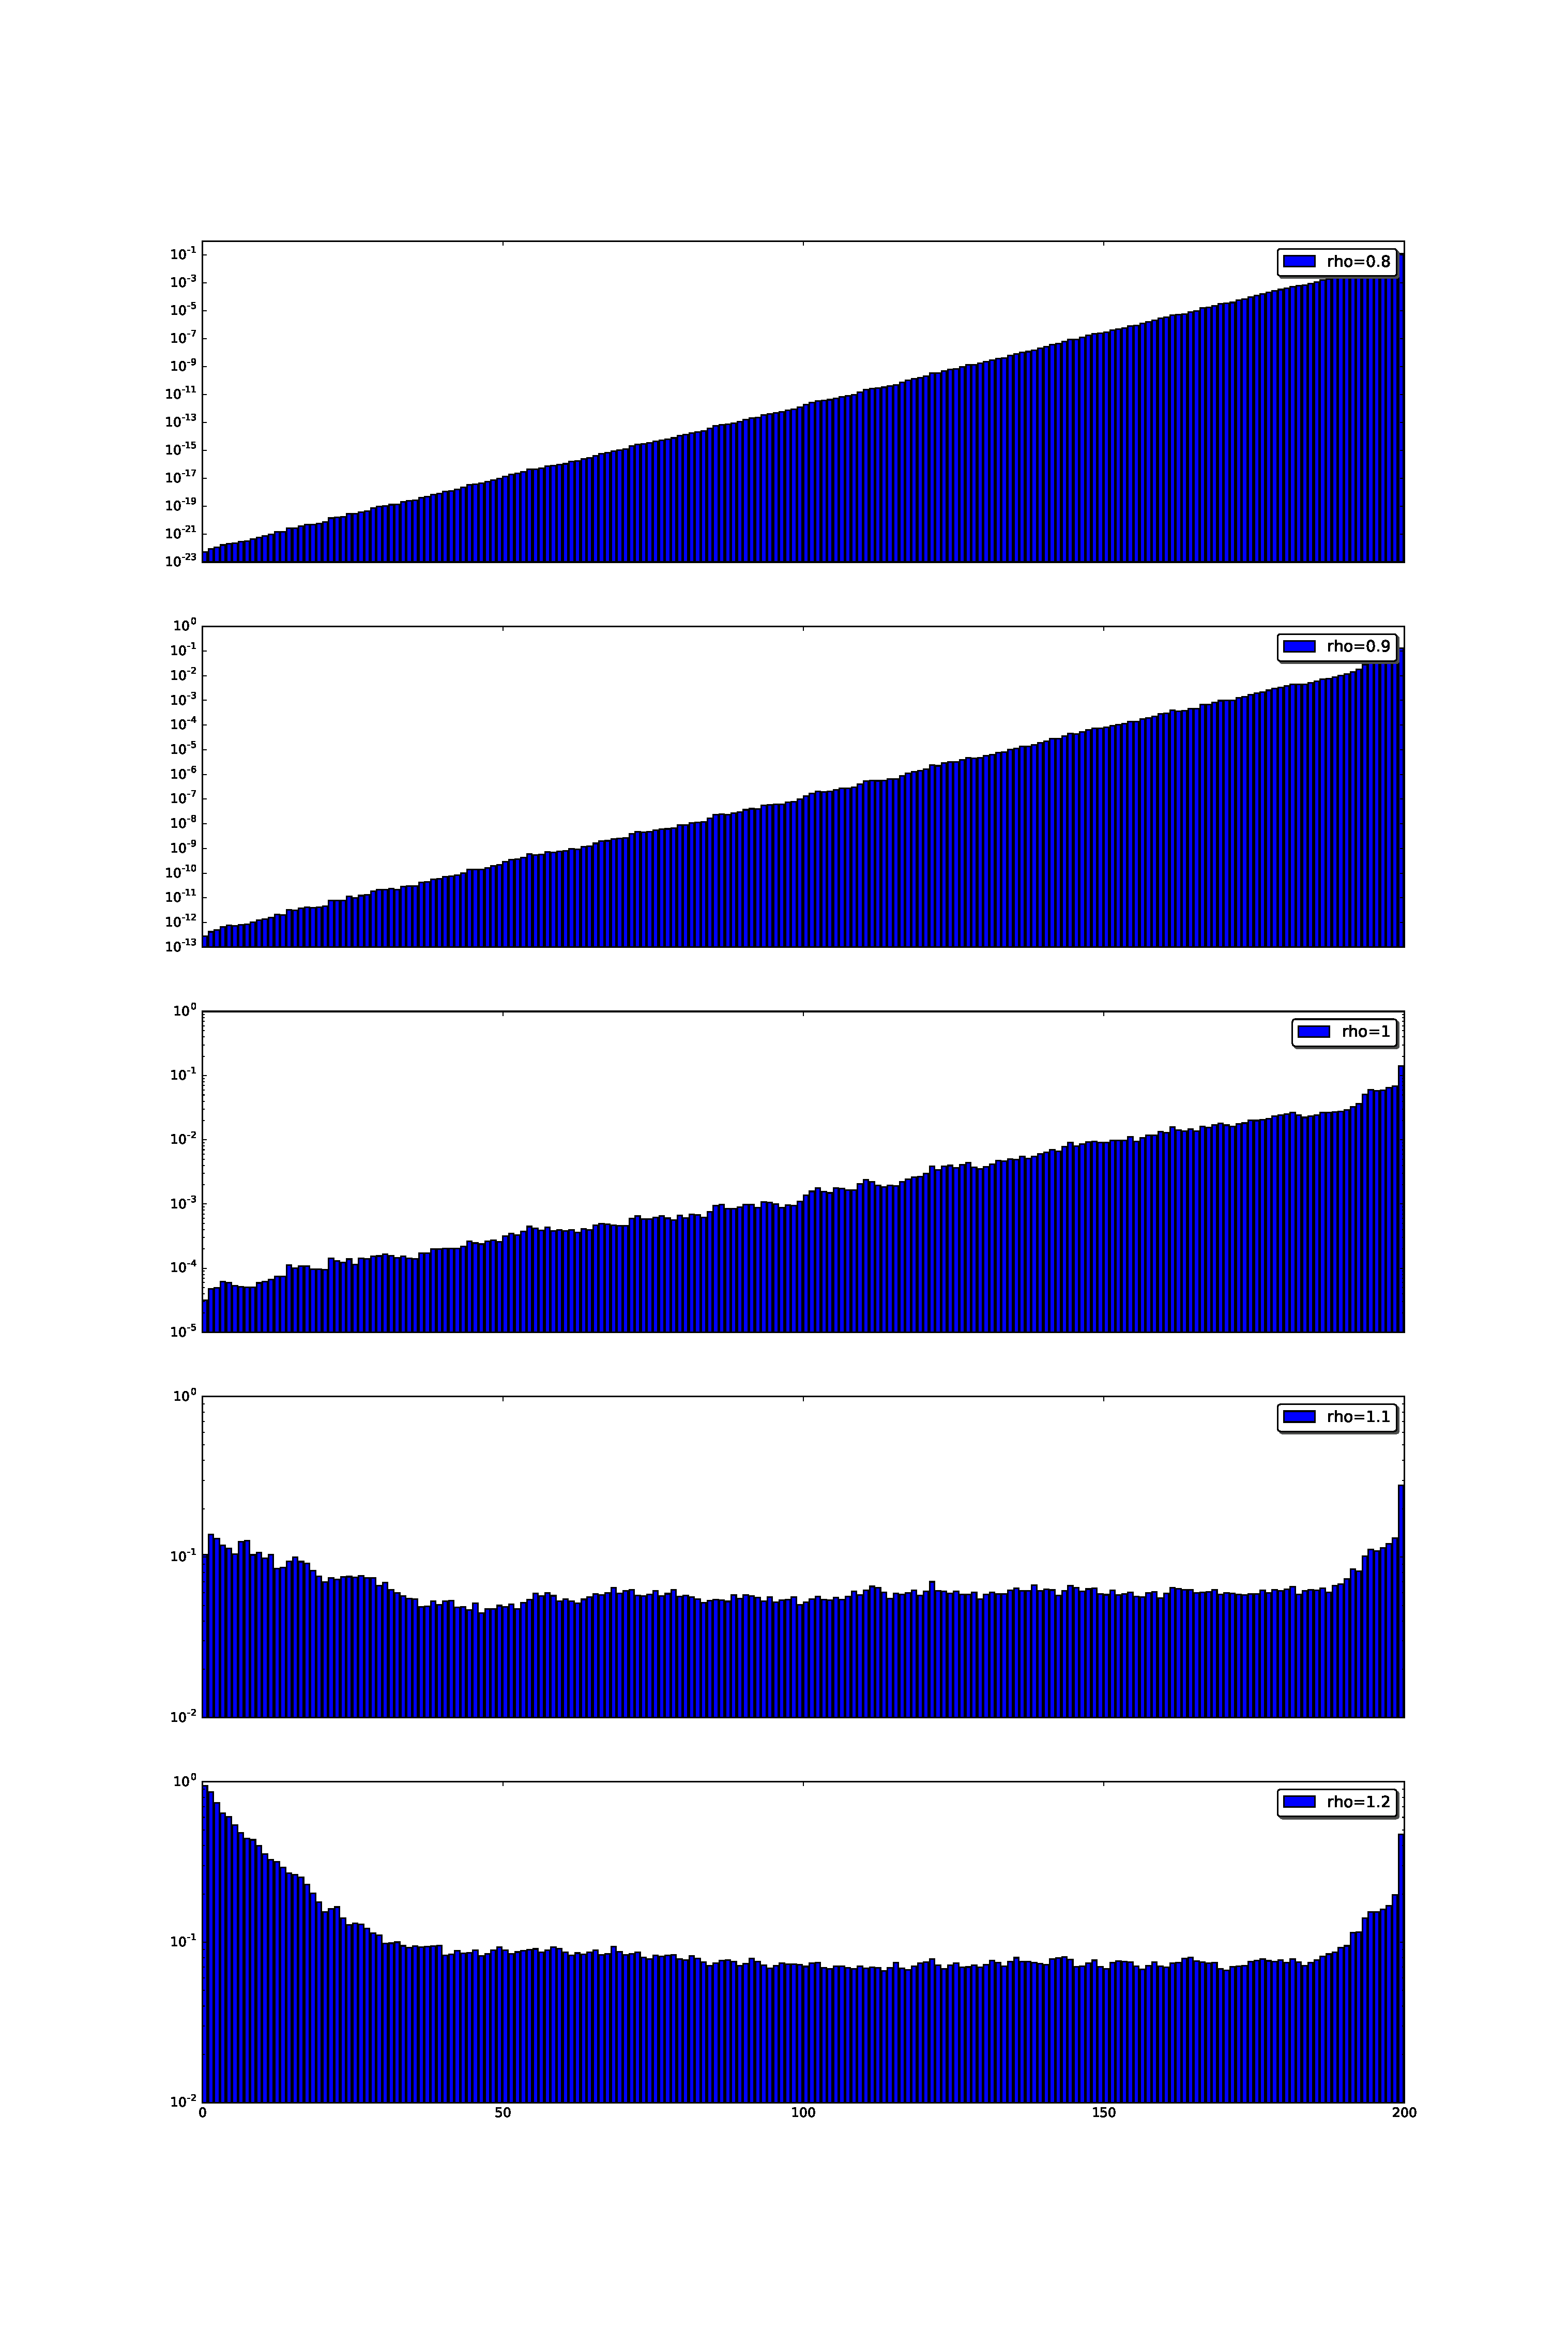
\includegraphics[width=0.6\textwidth]{temporal_components_rho.eps}
		\caption{Temporal gradients for the temporal order task varying the spectral radius of the recurrent matrix. y axis is in logarithmic scale.}
		\label{fig:temporal_norms}
	\end{figure}
\end{frame}

\begin{frame}{Effect of initialization on the rate of success}
	\begin{figure}
		\centering
		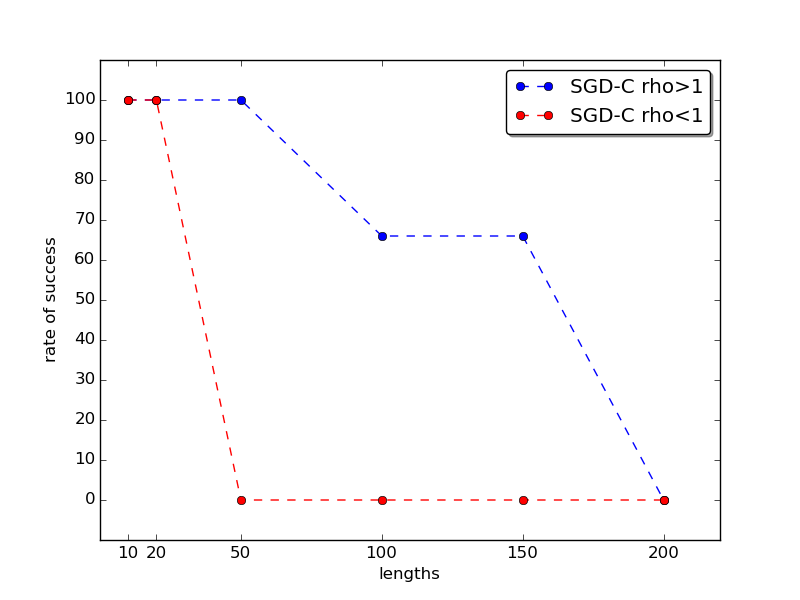
\includegraphics[width= 0.7\textwidth]{temporal_rates.png}
		\caption{Rate of success (mean of 3 runs) for the temporal order task for various lengths with SGD modified with gradient clipping. In blue and red the results when $W_{rec}$ is initialized with spectral radius bigger and smaller than one respectively.}
		\label{fig:temporal_rates}
	\end{figure}
\end{frame}


\begin{frame}{A different descent direction}
	The idea is to use the structure of the gradient to compute a "descent" direction which does not suffer from the vanishing problem.
\begin{itemize}
	\item Normalize the temporal gradients:
	\begin{equation}
	s_t(\vec{x}) = \frac{\nabla L_{|t}(\vec{x})}{\norm{\nabla L_{|t}(\vec{x})}}.
	\end{equation}
	
	\item Combine the normalized gradients in a convex way:
	\begin{equation}
	s(\vec{x}) = \sum_{t=1}^T \beta_t \cdot s_t(\vec{x}).
	\end{equation}
	
	with $\sum_{t=1}^T\beta_t=1, \beta_t>0$ (randomly picked at each iteration).
	\item Introduce the gradient norm:
	\begin{equation}
	d(\vec{x}) = - \norm{\nabla L (\vec{x})}\frac{s(\vec{x})}{\norm{s(\vec{x})}}.
	\end{equation}
\end{itemize}
\end{frame}

\begin{frame}{}
	\begin{center}
		\scalebox{0.65}{
			\begin{minipage}{0.8\linewidth}
\begin{algorithm}[H]
	\KwData{\\
		\Indp
		$D=\{\pair{\vec{x}^{(i)}}{\vec{y}^{(i)}}\}$: training set\\
		$m$: size of each mini-batch\\
		$\mu$: constant learning rate\\
		$\tau$: gradient clipping threshold \\
		$\rho$: initial spectral radius \\
		$\psi$ threshold for the direction norm
	}
	
	
	$\mat{W_{rec}}, \mat{W_{in}, \mat{W_{out}}} \sim \mathcal{N}(0, \sigma^2)$\\
	$\vec{b}_{out}, \vec{b}_{rec} \gets 0$\\
	$r \gets \mbox{spectral\_radius}(\mat{W_{rec}})$\\
	$\mat{W_{rec}}\gets \frac{\rho}{r} \cdot \mat{W_{rec}}$\\
	$\theta_0 = [\mat{W_{rec}}, \mat{W_{in}}, \mat{W_{out}},\vec{b}_{out}, \vec{b}_{rec}]$
	
	
	\BlankLine
	\While{stop criterion}{
		
		$I$ $\gets$ sample $m$ training example $\in D$  \\
		$\{\nabla_\theta L_{|t}\}_{t=1}^{T} \gets \mbox{compute\_temporal\_gradients}(\theta_k, I)$\\
		$\vec{d}_k \gets \mbox{simplex\_combination}(\{\nabla_\theta L_{|t}\})$\\
		
		\If{$\norm{\nabla_{\theta}L(\theta_k)}_2 > \psi$}
		{$\vec{d}_k \gets \nabla_{\theta}L(\theta_k)$ \\
			\label{algo:line:condition}
		}
		
		$\alpha_k = 
		\begin{cases}
		\mu  \quad &\mbox{if} \norm{\vec{d}_k}_2 \leq \tau\\
		\frac{\mu \cdot \tau}{\norm{\vec{d}_k}_2} \quad & \mbox{otherwise}
		\end{cases}$\\
		
		$\theta_{k+1} \gets \theta_k + \alpha_k \vec{d}_k$\\
		$k\gets k+1$
	}
	\KwRet{$\theta_k$}
	\caption{RNN training}
	\label{algo:complete_solution}
\end{algorithm}
\end{minipage}%
}
\end{center}

\end{frame}

\begin{frame}{Effect of the simplex direction}
	
	\begin{figure}
		\centering
	     \subfloat[][ Loss (in log scale) for the addition task during training]{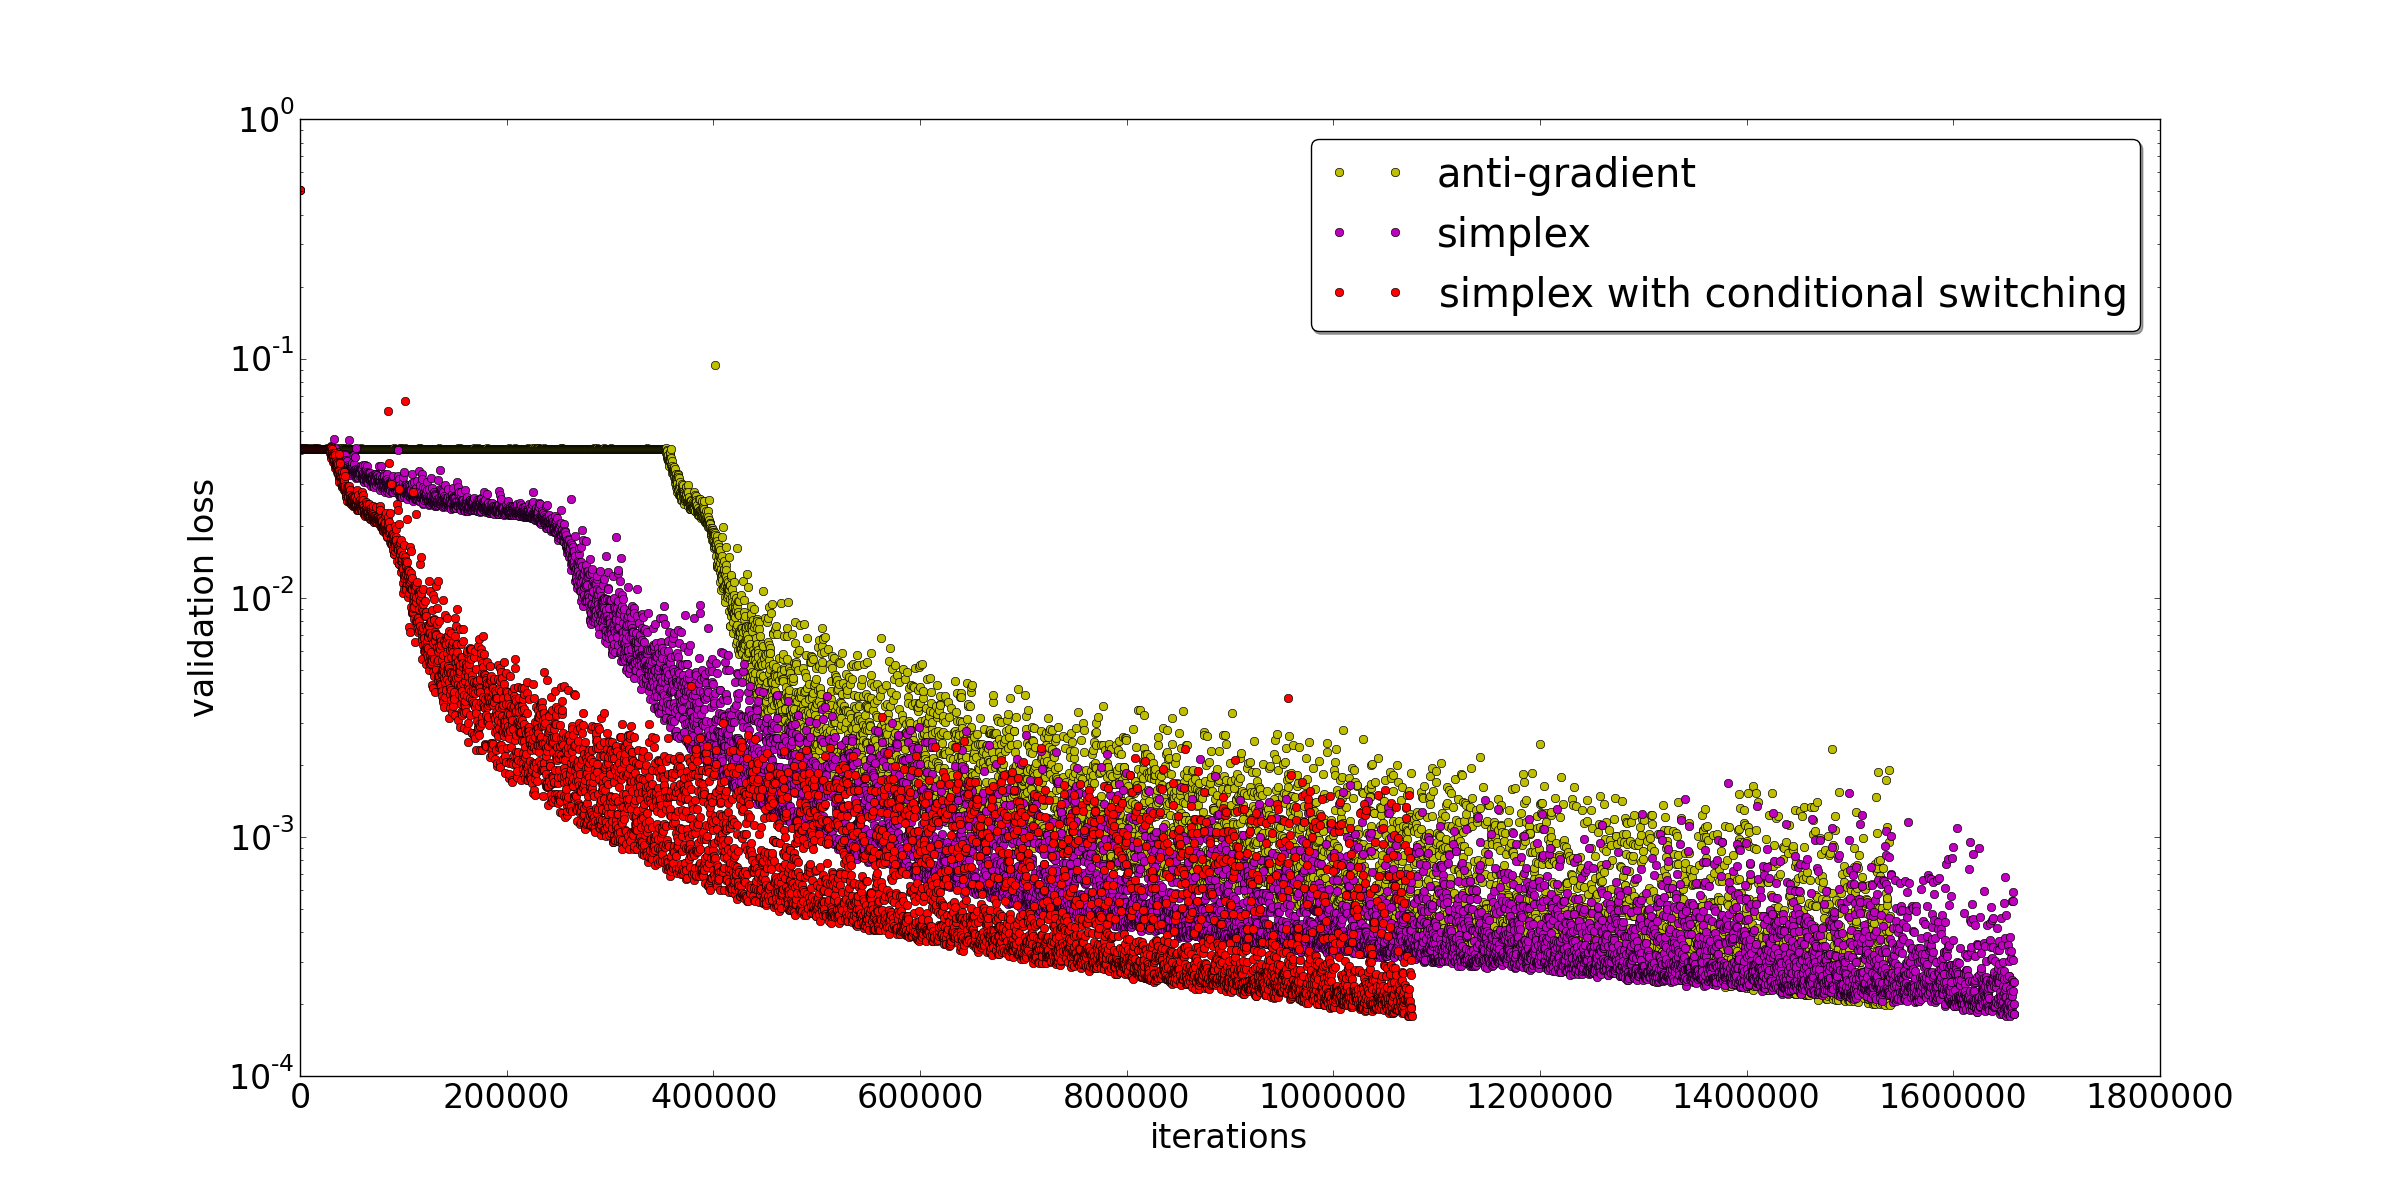
\includegraphics[width= 0.55\textwidth]{compare_add_simplex_13.png}\label{fig:compare_add_13}}
	     \subfloat[][Number of iterations]{\raisebox{3em}{\resizebox{0.5\columnwidth}{!}{
	     		{\renewcommand{\arraystretch}{1.3}
	     		\begin{tabular}[b]{C{3cm} | C{2cm} C{4cm}}
	     		& anti-gradient & simplex with conditional switching \\
	     		\hline
	     		addition & 1807466 & \textbf{1630666} \\
	     		temporal order & 	2164800 & \textbf{1010000}\\
	     	\end{tabular}}}
	     }
	    }
		\caption{Comparison between SGD using as descent direction the anti-gradient, the simplex direction and the simplex direction with conditional switching.}
		\label{fig:1}
	\end{figure}
	
%	\begin{figure}[h]
%		\begin{subfigure}{1.\textwidth}
%			\centering
%			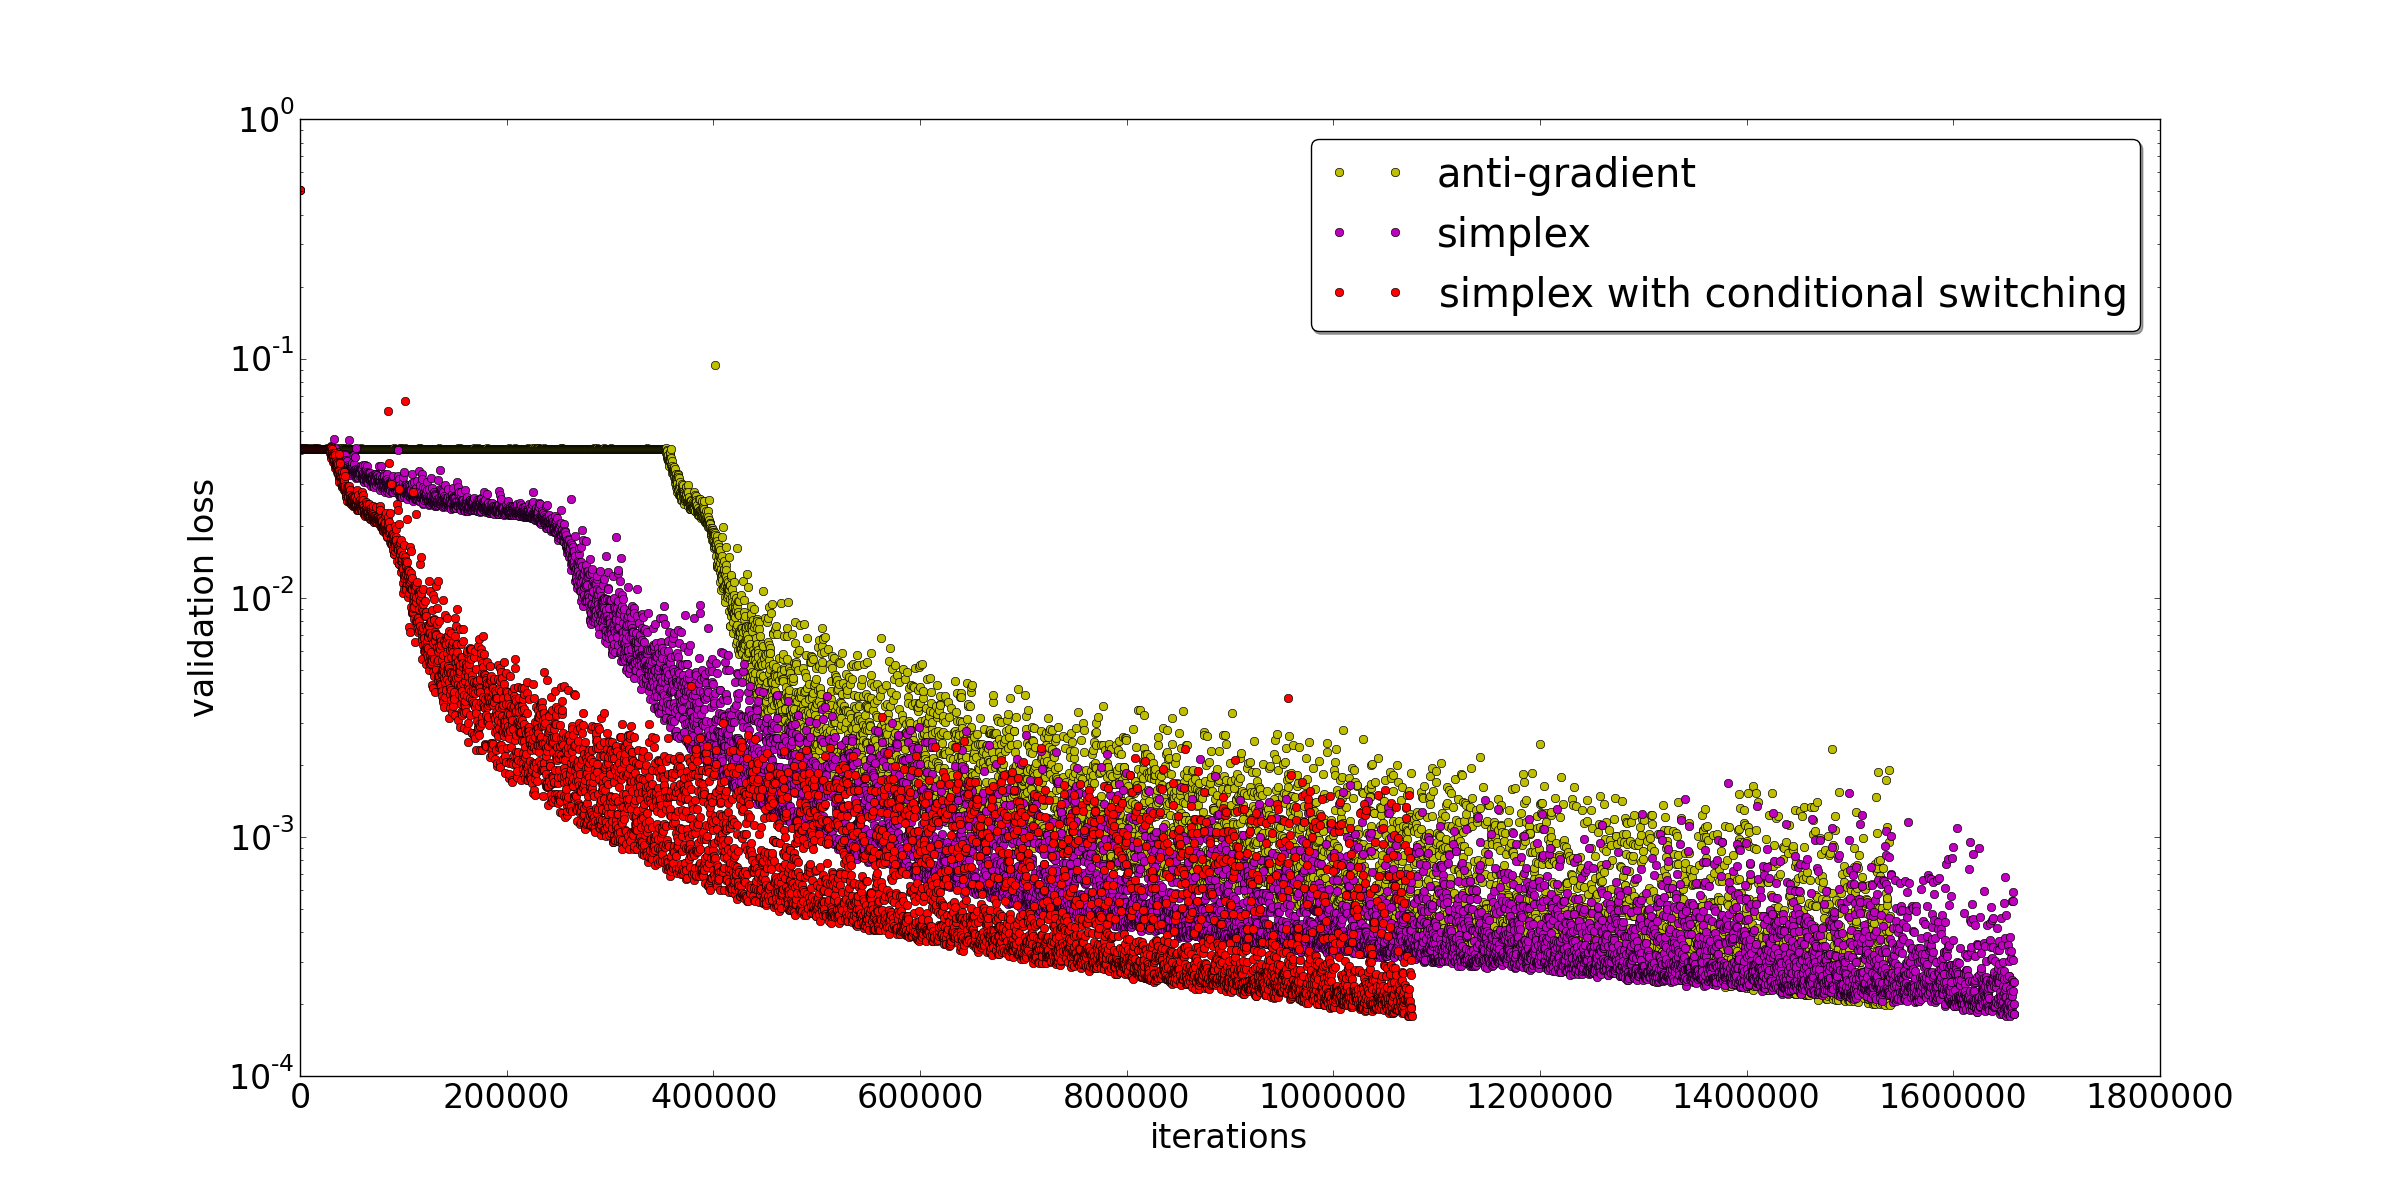
\includegraphics[width= 1\textwidth]{compare_add_simplex_13.png}
%			\caption{First run}
%			\label{fig:a:comparisong_add_simplex}
%		\end{subfigure}\\
%		\begin{subfigure}{1.\textwidth}
%			\centering
%			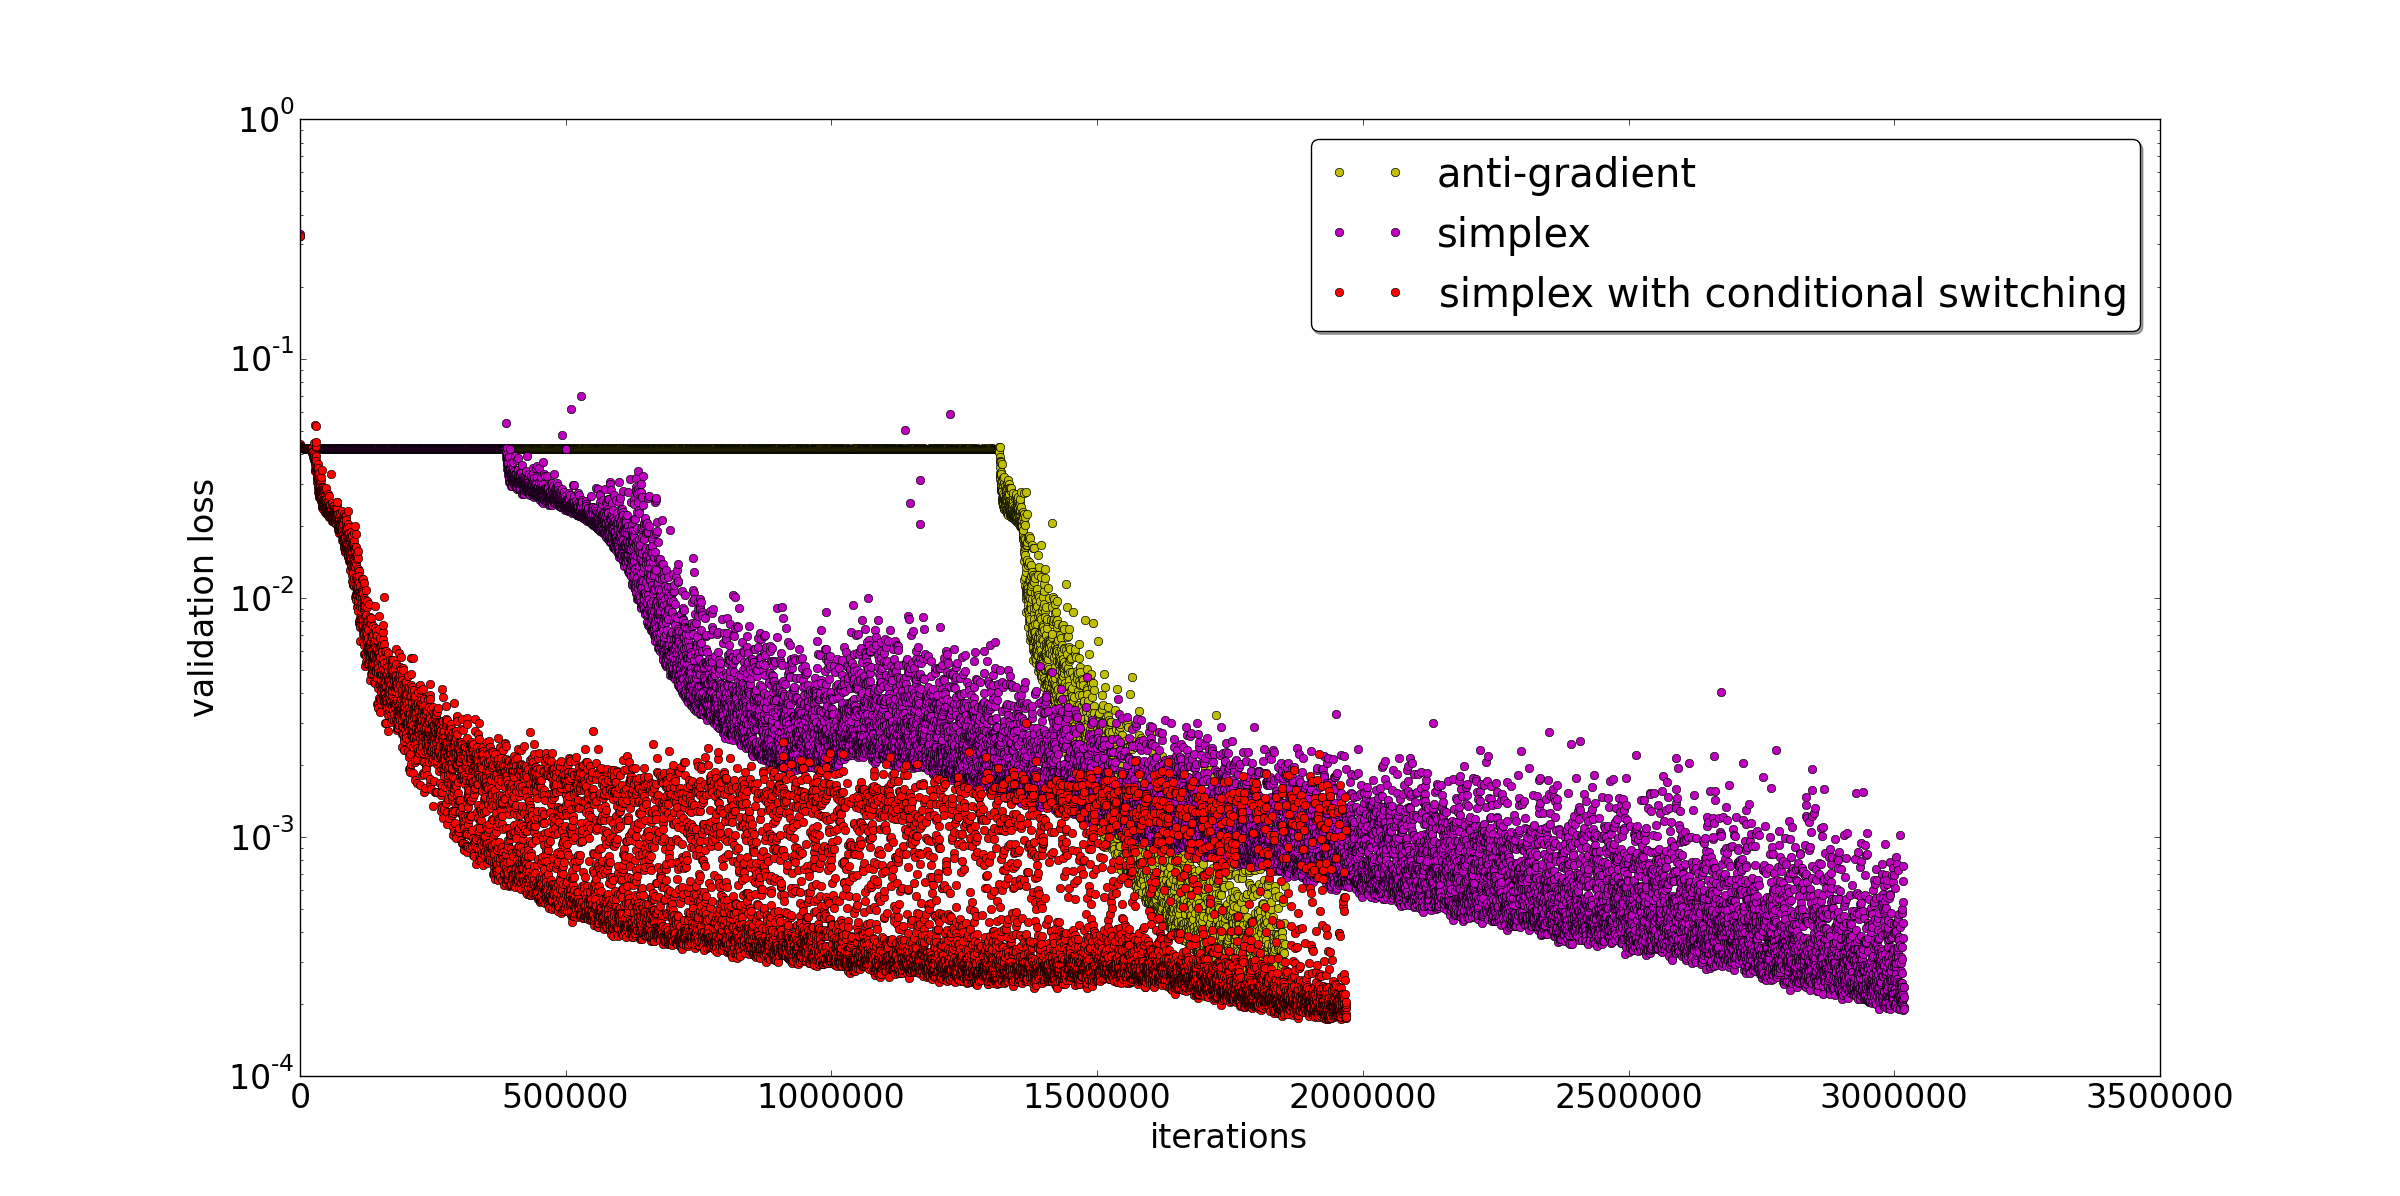
\includegraphics[width= 1\textwidth]{compare_add_simplex_14.png}
%			\caption{Second run}
%			\label{fig:b:comparisong_add_simplex}
%		\end{subfigure}\\
%		\begin{subfigure}{1.\textwidth}
%			\centering
%			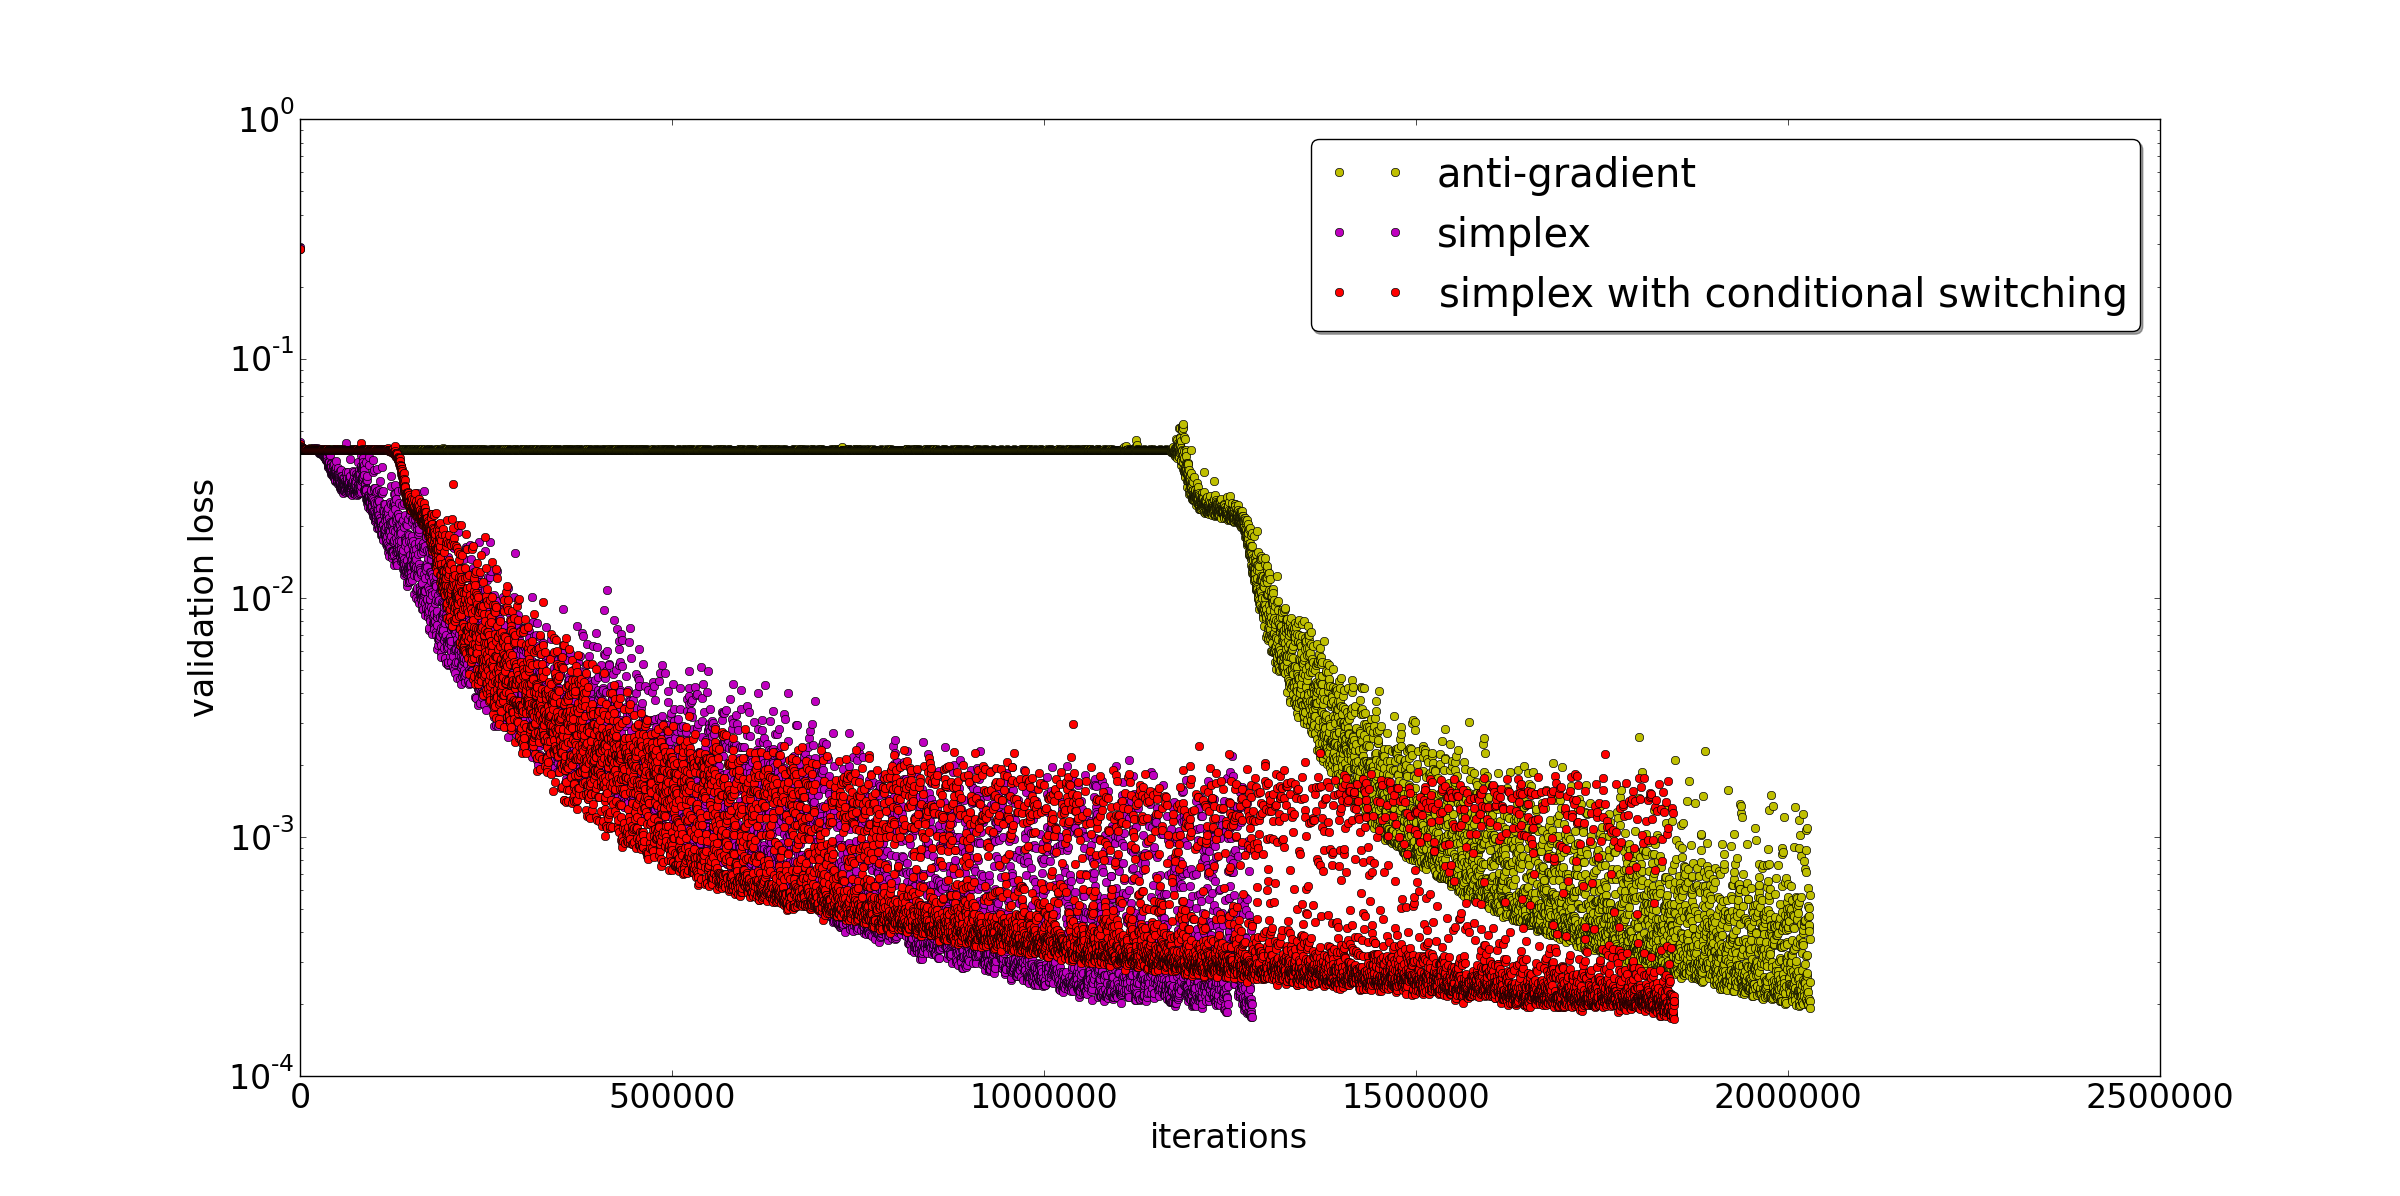
\includegraphics[width= 1\textwidth]{compare_add_simplex_15.png}
%			\caption{Third run}
%			\label{fig:c:comparisong_add_simplex}
%		\end{subfigure}%
%		\caption{Comparison between SGD using as descent direction the anti-gradient (in yellow, start decreasing always for last), the simplex direction (in purple, which is the second that start decreasing) and the simplex direction with conditional switching (in red, start decreasing always for first) for the addition task (T=100). In y axis the loss (mean squared error) in logarithmic scale.}
%		\label{fig:comparisong_add_simplex}
%	\end{figure}
\end{frame}
